\documentclass[a4paper,14pt]{extarticle}

\usepackage[utf8x]{inputenc}
\usepackage[T1,T2A]{fontenc}
\usepackage[russian]{babel}
\usepackage{hyperref}
\usepackage{indentfirst}
\usepackage{here}
\usepackage{array}
\usepackage{graphicx}
\usepackage{caption}
\usepackage{subcaption}
\usepackage{chngcntr}
\usepackage{amsmath}
\usepackage{amssymb}
\usepackage{pgfplots}
\usepackage{pgfplotstable}
\usepackage[left=2cm,right=2cm,top=2cm,bottom=2cm,bindingoffset=0cm]{geometry}
\usepackage{multicol}

\renewcommand{\le}{\ensuremath{\leqslant}}
\renewcommand{\leq}{\ensuremath{\leqslant}}
\renewcommand{\ge}{\ensuremath{\geqslant}}
\renewcommand{\geq}{\ensuremath{\geqslant}}
\renewcommand{\epsilon}{\ensuremath{\varepsilon}}
\renewcommand{\phi}{\ensuremath{\varphi}}

\counterwithin{figure}{section}
\counterwithin{equation}{section}
\counterwithin{table}{section}
\newcommand{\sign}[1][5cm]{\makebox[#1]{\hrulefill}} % Поля подписи и даты
\graphicspath{{pics/}} % Путь до папки с картинками
\captionsetup{justification=centering,margin=1cm}
\def\arraystretch{1.3}

\usepackage{courier}

\usepackage{listings}
\lstset{ %
extendedchars=\true,
keepspaces=true,
language=C,						% choose the language of the code
basicstyle=\footnotesize,		% the size of the fonts that are used for the code
numbers=left,					% where to put the line-numbers
numberstyle=\footnotesize,		% the size of the fonts that are used for the line-numbers
stepnumber=1,					% the step between two line-numbers. If it is 1 each line will be numbered
numbersep=5pt,					% how far the line-numbers are from the code
backgroundcolor=\color{white},	% choose the background color. You must add \usepackage{color}
showspaces=false				% show spaces adding particular underscores
showstringspaces=false,			% underline spaces within strings
showtabs=false,					% show tabs within strings adding particular underscores
frame=single,           		% adds a frame around the code
tabsize=2,						% sets default tabsize to 2 spaces
captionpos=b,					% sets the caption-position to bottom
breaklines=true,				% sets automatic line breaking
breakatwhitespace=false,		% sets if automatic breaks should only happen at whitespace
escapeinside={\%*}{*)},			% if you want to add a comment within your code
postbreak=\raisebox{0ex}[0ex][0ex]{\ensuremath{\color{red}\hookrightarrow\space}},
texcl=true,
}

\lstset{basicstyle=\footnotesize\ttfamily,breaklines=true}

\begin{document}

\begin{titlepage}
\begin{center}
	\textbf{Санкт-Петербургский Политехнический Университет \\Петра Великого}\\[0.3cm]
	\small Институт компьютерных наук и технологий \\[0.3cm]
	\small Кафедра компьютерных систем и программных технологий\\[4cm]
	
	\textbf{ОТЧЕТ}\\ \textbf{о лабораторной работе}\\[0.5cm]
	\textbf{<<Использование стандартных подпрограмм для приближенного\\ вычисления интеграла>>}\\[0.1cm]
	\textbf{Вычислительная математика}\\[8.0cm]
\end{center}

\begin{flushright}
	\begin{minipage}{0.48\textwidth}
		\begin{flushleft}
			\small \textbf{Работу выполнил студент}\\[3mm]
			\small группа 23501/4 \hspace*{6mm} Дьячков В.В.\\[5mm]
			
			\small \textbf{Преподаватель}\\[5mm]
		 	\small \sign[3cm] \hspace*{5mm} к.т.н., доц. Цыган В.Н.\\[0.5cm]
		\end{flushleft}
	\end{minipage}
\end{flushright}

\vfill

\begin{center}
	\small Санкт-Петербург\\
	\small \the\year
\end{center}
\end{titlepage}

\section{Техническое задание}

\textbf{Задание К-3-08:} Дана консольная балка с переменным поперечным сечением, показанная на рисунке \ref{img:balka}.

\begin{figure}[H]
\begin{center}
	\vspace{-0.5cm}
	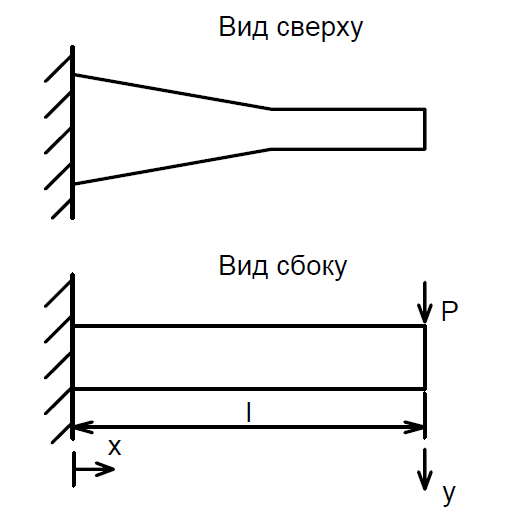
\includegraphics[scale=0.45]{balka}
	\caption{Консольная балка}
	\label{img:balka}
	\vspace{-0.5cm}
\end{center}
\end{figure}

Дифференциальное уравнение для вертикального прогиба имеет вид:
\begin{equation}\label{eq:diff}
	\frac{d^4y}{dx^4} = - \frac{2}{I} \frac{dI}{dx}\cdot \frac{d^3y}{dx^3} -  \frac{1}{I} \frac{d^2I}{dx^2}\cdot \frac{d^2y}{dx^2} + \frac{\omega}{EI},
\end{equation}

где $x$ -- горизонтальное расстояние вдоль балки, $y$ -- вертикальный прогиб, $l$ -- длина балки, $M$ -- изгибающий момент, $E$ -- модуль Юнга, $I$ -- момент инерции, $P$ -- нагрузка на балку.

\begin{center}
\begin{multicols}{2}
$\omega = - \frac{d^2M}{dx^2}$\\
$M(x) = -P \cdot (l - x)$
\end{multicols}
\end{center}

\begin{center}
\begin{multicols}{2}
$E = 3\cdot 10^7$\\
$I(x) = 5 \cdot (1 + 4 e^{-\frac{6x}{l}})$
\end{multicols}
\end{center}

Начальные условия:
\begin{center}
\begin{multicols}{3}
$y(0) = y'(0) = 0$\\
$y''(0) = \frac{Pl}{75}\cdot 10^{-7}$\\
$y'''(0) = \frac{P \cdot 3.8}{75}\cdot 10^{-7}$
\end{multicols}
\end{center}

Вычислить $y(l)$ для различных значений $P$. Построить сплайн по значениям $y(l)$ в зависимости от $P$ и с его помощью оценить $y(l)$ для $P_0$. 

Оценить погрешность результата и влияние на точность погрешности исходных данных.

\section{Исходные данные}

Значения нагрузки на балку: 
\begin{equation}\label{eq:p_values}
	500 \le P \le 1000 \text{ с шагом } 100,\ P_0 = 750.
\end{equation}

Значения длины балки: $l = 50\cdot x^*$, где $x^*$ -- корень уравнения \ref{eq:int} на промежутке $[1, 4]$.

\begin{equation}\label{eq:int}
	\int_0^{20} \frac{e^{-0.9z}}{z+x}dz = 0.1957981\cdot x
\end{equation}

\section{Инструменты разработки}

Задание было выполнено с использованием языка программирования \textbf{Python}. Это мощный инструмент для создания программ самого разнообразного назначения, в том числе для построения и анализа математических моделей. Python является интерпретируемым языком, а к его основным особенностями относятся динамическая типизаця, автоматическая сборка мусора, позволяющая избежать утечек памяти, и кроссплатформенность. 

В процессе работы также использовалась популярная бесплатная интерактивная оболочка для этого языка программирования \textbf{Jupyter} Notebook, позволяющая объединить код, изображения, комментарии, формулы и графики. Раньше она называлась IPython Notebook, но название было изменено, чтобы подчеркнуть совместимость не только с Python, но и другими языками программирования. Основные отличительные особенности данной платформы  это комплексная интроспекция объектов, т.е. возможность определить тип и структуру объекта во время выполнения программы, сохранение истории ввода на протяжении всех сеансов, кэширование выходных результатов, подсветка синтаксиса и удобное совмещение математического описания модели в виде текста и формул с кодом программы, описывающей данную модель. 

К преимуществам же самого языка, помимо перечисленных, стоит отнести понятный и лаконичный синтаксис, способствующий ясному отображению кода, огромное количество модулей, как входящих в стандартную поставку Python, так и сторонних, что позволяет решать огромный спектр задач, используя уже написанный код. В частности, модуль \textbf{SciPy} содержит большое количество функций, позволяюших решать множество задач вычислительной математики: от решения нелинейных уравнений и интерполяции функции до вычисления интегралов и решения систем дифференциальных уравнений.

\section{Выполнение работы}

\subsection{Анализ исходного уравнения}

Последнее слагаемое исходного дифференциального уравнения:
\[
	\omega = -\frac{d^2M}{dx^2},\ \ \ M(x) = -P \cdot (l - x).
\]

Можно заметить, что $\frac{d^2M}{dx^2} = 0$ при $\forall x$, а значит и $\frac{\omega}{EI} = 0$ при $\forall x$.

Таким образом дифференциально уравнение \ref{eq:diff} преобразуется к виду:
\begin{equation}\label{eq:source}
	\frac{d^4y}{dx^4} = - \frac{2}{I} \frac{dI}{dx}\cdot \frac{d^3y}{dx^3} - \frac{1}{I} \frac{d^2I}{dx^2}
\end{equation}

Были вычислены производные функции $I(x)$:
\begin{multicols}{2}
\noindent
\[
	\frac{dI}{dx} = -\frac{120}{l}e^{-\frac{6x}{l}}
\]
\[
	\frac{d^2I}{dx^2} = \frac{720}{l}e^{-\frac{6x}{l}}
\]
\end{multicols}

Найденные значения можно подставить в уравнение \ref{eq:source}:
\begin{equation}
\frac{d^4y}{dx^4} = \frac{2}{5(1 + 4e^{-\frac{6x}{l}})} \cdot \frac{120}{l}e^{-\frac{6x}{l}} \cdot \frac{d^3y}{dx^3} - 
\frac{1}{5(1 + 4e^{-\frac{6x}{l}})} \cdot \frac{720}{l}e^{-\frac{6x}{l}} \cdot \frac{d^2y}{dx^2}
\end{equation}

\subsection{Нахождение длины балки}

По условию задачи длина балки $l = 50\cdot x^*$, где $x^*$ - корень уравнения \ref{eq:int} на промежутке $[1, 4]$. Для решения задачи была задана следующая функция:
\begin{equation}
F(x) = \int_0^{20} \frac{e^{-0.9z}}{z+x}dz - 0.1957981\cdot x
\end{equation}

Затем для нахождения корней функция $F(x)$ с начальным приближением $x = 2.5$ была использована функция \textbf{optimize.fsolve} из модуля \textbf{SciPy}, являющаяся оберткой над алгоритмами \textsc{hybrd} и \textsc{hybrj} из библиотеки \textsc{minpack} для языка программирования \textsc{fortran}. 

Для интегрирования использовалась функция \textbf{integrate.quad} из модуля \textbf{SciPy}, применяющая технику из библиотеки \textsc{quadpack} для того же языка программирования.

Найденный корень $x^* \approx 1.999696$, следовательно длина балки 
$l \approx 99.984776$.

\subsection{Решение дифференциального уравнения}

Исходное дифференциальное уравнение при помощи подстановок \ref{eq:subs} было приведено к системе дифференциальных уравнений первого порядка \ref{eq:system}:
\begin{equation}\label{eq:subs}
x_1(t) = y(t),\ \ \ x_2(t) = y'(t),\ \ \ x_3(t) = y''(t),\ \ \ x_4(t) = y'''(t)
\end{equation}

\begin{equation}\label{eq:system}
\begin{pmatrix}
    x'_1(t) \\
    x'_2(t) \\
    x'_3(t) \\
    x'_4(t) \\
\end{pmatrix} =
\begin{pmatrix}
    0 & 1 & 0 & 0 \\
    0 & 0 & 1 & 0 \\
    0 & 0 & 0 & 1 \\
    0 & 0 & - \frac{1}{I} \frac{d^2I}{dx^2} & - \frac{2}{I} \frac{dI}{dx} \\
\end{pmatrix}
\cdot
\begin{pmatrix}
    x_1(t) \\
    x_2(t) \\
    x_3(t) \\
    x_4(t) \\
\end{pmatrix}
\end{equation}

\begin{figure}[H]
\begin{center}
	\vspace{-0.5cm}
	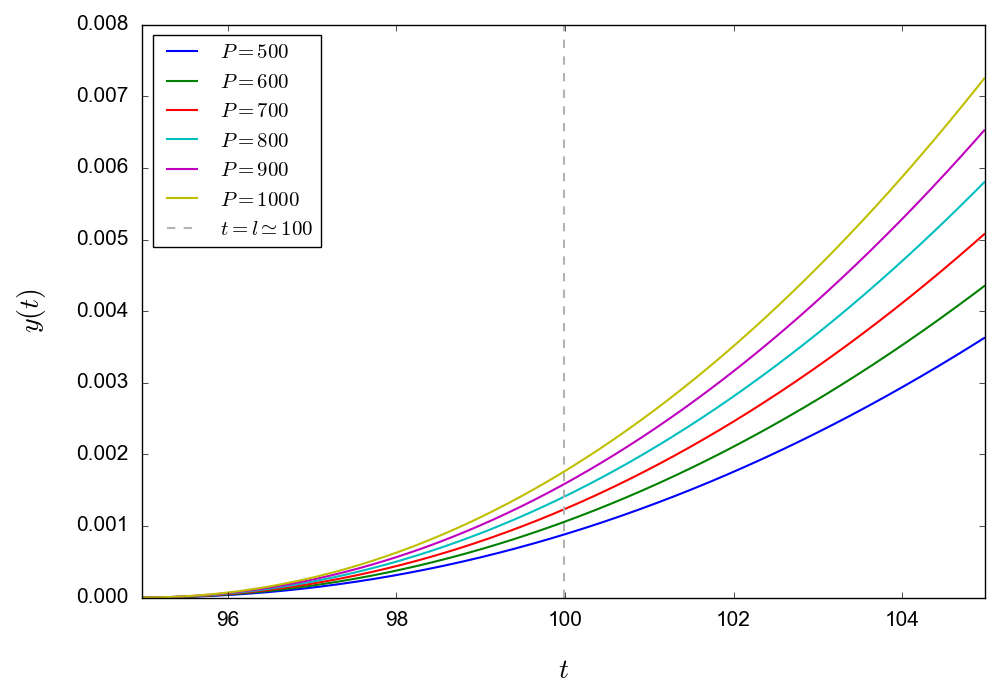
\includegraphics[scale=0.6]{p}
	\caption{Зависимость $y(t)$ для различных значений $P$}
	\label{plt:p}
	\vspace{-0.5cm}
\end{center}
\end{figure}

При решении дифференциального уравнения использовалась функция \textbf{integrate.odeint} из модуля \textbf{SciPy}, которая применяет алгоритм \textsc{lsoda} из библиотеки \textsc{odepack} для языка программирования \textsc{fortran}.

Для каждого значения нагрузки на балку из исходных данных \ref{eq:p_values} была решена система дифференциальных уравнений первого порядка \ref{eq:system} в диапазоне $(l-5) \div (l+5)$ с шагом $0.01$.

На рисунке \ref{plt:p} изображена полученная зависимость $y(t)$ от независимой переменной $t$ для различных значений $P$. Пунктирной линией на графике показана прямая $t = l$.

\subsection{Нахождение значения $y(l)$ при $P = P_0$}

По значениям $y(l)$ при различных значениях P была построена кубическая интерполяция $S(P)$ и найдено значение $S(P_0) = S(750)$.

Для интерполяции была использована функция \textbf{interpolate.interp1d} с параметром \texttt{'cubic'} из модуля \textbf{SciPy}, которая использует алгоритм из библиотеки \textsc{fitpack} для языка программирования \textsc{fortran}.

По найденному сплайну было найдено значение $S(P_0) \approx 0.001317$.

\begin{figure}[H]
\begin{center}
	\vspace{-0.5cm}
	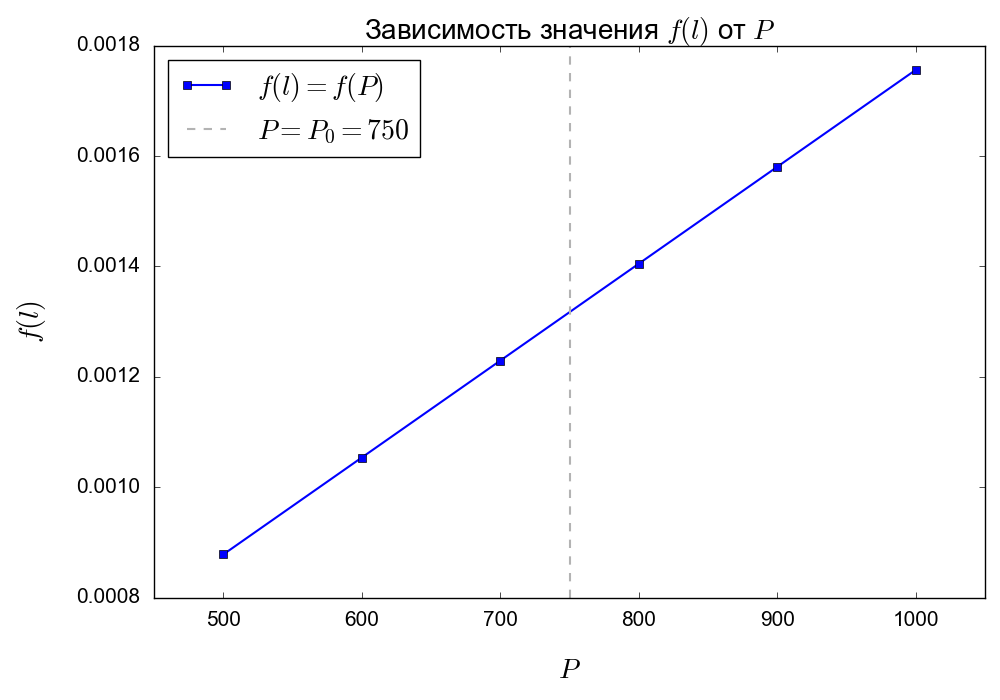
\includegraphics[scale=0.6]{l}
	\caption{Зависимость $f(l)$ от $P$}
	\label{plt:l}
	\vspace{-0.5cm}
\end{center}
\end{figure}

На рисунке \ref{plt:l} изображена полученная зависимость значения $f(l)$ от $P$. Пунктирной линией на граифке показана прямая $P = P_0 = 750$.

\subsection{Анализ влияния погрешности начальных условий на решение}

Влияние погрешностей начальных условий было проанализировано при помощи варьирования коэффициентов в функции момента инерции $I(x)$:
\begin{equation}\label{eq:var}
I(x) = \alpha \cdot(1 + 4e^{-\frac{\beta\cdot x}{l}})
\end{equation}

Коэффициенты $\alpha$ и $\beta$ изменялись в пределах $\pm 10\ \%$ с шагом $h = 0.01$, нагрузка на балку при этом была задана $P = P_0 = 750$:
\begin{multicols}{2}
\noindent
\[
	\alpha = \alpha_0 \pm 0.1\cdot \alpha_0 = 5 \pm 0.5 = 4.5 \div 5.5
\]
\[
	\beta = \beta_0 \pm 0.1\cdot \beta_0 = 6 \pm 0.6 = 5.4 \div 6.6
\]
\end{multicols}

Для оценки влияния параметра на решение была введена функция $\epsilon(a, b)$, равная модулю разности найденного значения $y_{\alpha_0\beta_0}(l) = S(P_0)$ и значения $y_{ab}(l)$, полученного при подстановке в уравнение \ref{eq:var} коэффициентов $\alpha = a$ и $\beta = b$:
\begin{equation}
	\epsilon(a, b) = |\ y_{\alpha_0\beta_0}(l) - y_{ab}(l)\ |
\end{equation}

\begin{figure}[H]
\begin{center}
	\vspace{-1cm}
	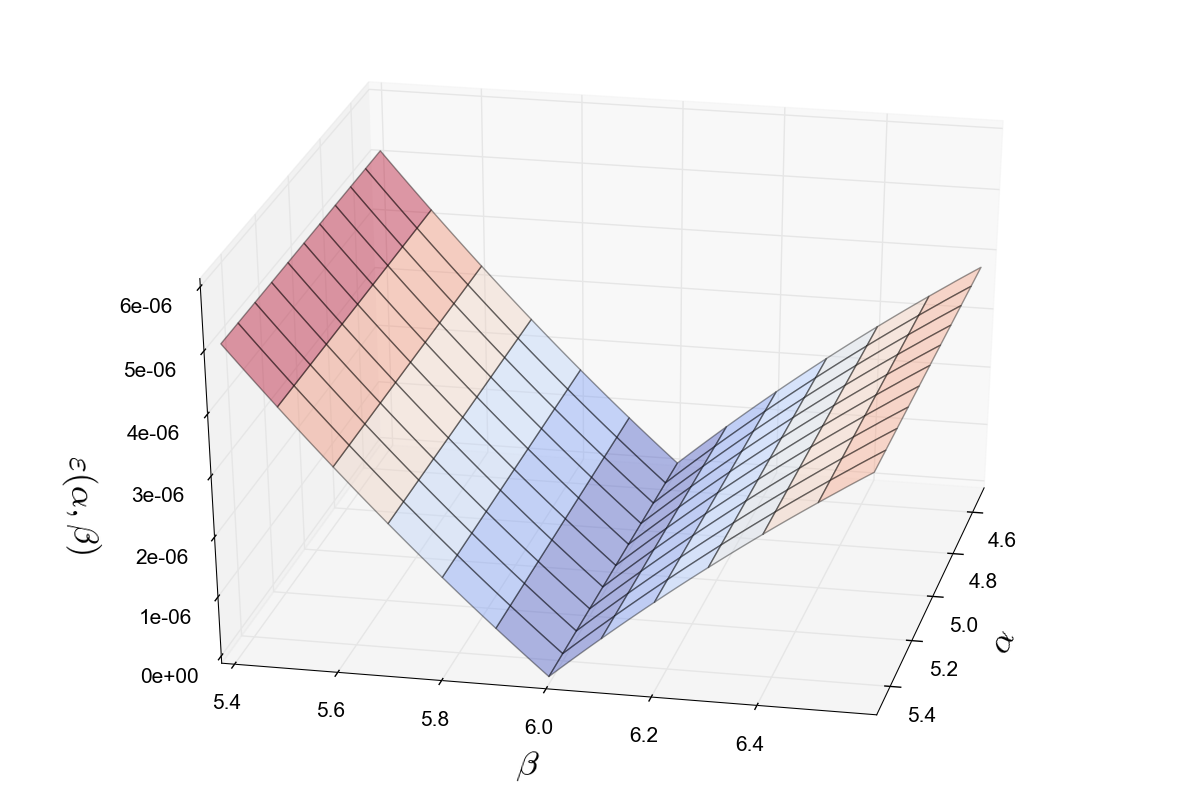
\includegraphics[scale=0.61]{ab}
	\caption{Зависимость $\epsilon$ от значений $\alpha$ и $\beta$}
	\label{plt:ab}
	\vspace{-0.5cm}
\end{center}
\end{figure}

На рисунке \ref{plt:ab} изображена полученная зависимость $\epsilon$ от различных значений $\alpha$ и $\beta$. Из построенного графика видно, что варьирование параметра  $\alpha$  в выбранном диапазоне имеет слабое влияение на итоговое решение, в то время как даже небольшое возмущение параметра  $\beta$  в аналогичном диапазоне приводит к более заметному изменению итогового результата.

\section{Результаты}

В ходе работы была найдена длина балки, решено дифференциальное уравнение, описывающее вертикальный прогиб балки, был построен сплайн по значениям $y(l)$ в зависимости от $P$ и с его помощью оценено значение $y(l)$ для $P_0$, а также исследовано влияние точности исходных данных на решение. Полученная информация позволила сделать выводы о влиянии точности задания коэффициентов в одном из начальных уравнений на получаемое решение.

\section*{Приложение}

\captionof{lstlisting}{coursework.py}
\lstinputlisting[language=Python,
	basicstyle=\scriptsize,	
	numberstyle=\scriptsize]{coursework.py}

\end{document}